%================================================================
% SLO
%----------------------------------------------------------------
% datoteka: 	thesis_template.tex
%
% opis: 		predloga za pisanje diplomskega dela v formatu LaTeX na
% 				Univerza v Ljubljani, Fakulteti za računalništvo in informatiko
%
% pripravili: 	Matej Kristan, Zoran Bosnić, Andrej Čopar,
%			  	po začetni predlogi Gašperja Fijavža
%
% popravil: 	Domen Rački, Jaka Cikač, Matej Kristan
%
% verzija: 		30. september 2016 (dodan razširjeni povzetek)
%================================================================


%================================================================
% SLO: definiraj strukturo dokumenta
% ENG: define file structure
%================================================================
\documentclass[a4paper, 12pt]{book}
 

%================================================================
% SLO: Odkomentiraj "\SLOtrue " za izbiro slovenskega jezika
% ENG: Uncomment "\SLOfalse" to chose English languagge
%================================================================
\newif\ifSLO
\newif\ifTRACKEXIST
\newif\ifTRACKCS
\newif\ifPROGRAMMM
\newif\ifPROGRAMEMAI


% ---------------------------------------------------------------------------------------
% IMPORTANT: Adjust the thesis language, your study program and track within this block
% ---------------------------------------------------------------------------------------
% ** switch language ** %
\SLOtrue % Enables Slovenian language
%\SLOfalse  % Enables English language

% ** Switch programs: ** %

% ** Uncomment if Program: Computer Science, Track: Computer Science **%
\TRACKCStrue
\TRACKEXISTtrue

% ** Uncomment if Program: Computer Science, Track: Data Science **%
%\TRACKCSfalse
%\TRACKEXISTtrue

% ** Uncomment if Program: Multimedia **%
%\PROGRAMMMtrue 
%\TRACKEXISTfalse 

% ** Uncomment if Program: EMAI **%
%\PROGRAMEMAItrue
%\SLOfalse 

% -------------------------------------------------------------------------------------------
% End of language, program and track adjustment
% -------------------------------------------------------------------------------------------


%================================================================
% SLO: vključi oblikovanje in pakete
% ENG: include design and packages
%================================================================
%----------------------------------------------------------------
% SLO: LaTeX paketi
% ENG: LateX packages
%----------------------------------------------------------------
% SLO: omogoča uporabo slovenskih (latinskih) črk kodiranih v formatu UTF-8
% ENG: enables the use of slovene (latin) caracters encoded in the UFT-8 format
\usepackage[utf8x]{inputenc}
%\inputencoding{utf8}
% SLO: naloži, med drugim, slovenske delilne vzorce
% ENG: loads, among others, slovene dividing patterns
\usepackage[slovene,english]{babel}
% SLO: poskrbi za postavitev strani
% ENG: takes care of the page layout
\usepackage{fancyhdr}
% SLO: za vlaganje slik različnih formatov
% ENG: for loading figures of different formats
\usepackage{graphicx}
\usepackage{caption}
\captionsetup[figure]{labelfont=bf} % SLO: napis "Slika #" v krepkem tisku
									% ENG: wirte "Figure #" caption in bold
\captionsetup[table]{labelfont=bf} % SLO: napis "Tabela #" v krepkem tisku
								   % ENG: wirte "Table #" caption in bold
% SLO: za pisanje psevdokode
% ENG: for writing pseudocode
\usepackage{algorithm}
\usepackage{algorithmic}
\floatname{algorithm}{\footnotesize Algorithm} % SLO: napis "Algoritem #" v krepkem tisku
											   % ENG: write "Algorithm #" caption in bold
% SLO: poveže reference slik/tabel in slike/tabele znotraj dokumenta
% ENG: links image/table references with the images/tables within the document
\usepackage[pdfa]{hyperref}
% SLO: pri kliku na referenco slike/tabele se postavi na vrh slike/tabele
% ENG: when clicking the image/table reference, position the focus on top of the image/table
\usepackage[all]{hypcap}
% SLO: omogoča, med drugim, definicjo in uporebo barve
% ENG: enables, among others, the definition and use of colors
\usepackage{xcolor}
%----------------------------------------------------------------
% SLO: dodatni paketi
% ENG: additional packages
%----------------------------------------------------------------
% SLO: omogoča večjo manipulacijo nad tabelami
% ENG: allows for greater manipulation of tables
\usepackage{booktabs}
% SLO: naloži dodatne simbole
% ENG: loads additional symbols
\usepackage{amssymb}
% SLO: omogoča, med drugim, sklicevanje na formule z eqref
% ENG: enables, among others, equation referencing with eqref
\usepackage{amsmath}
% SLO: omogoča komentiranje večjega dela teksta
% ENG: enables the commenting of larger text parts
\usepackage{verbatim}
% SLO: omogoča rotacijo PDF strani v ležeč položaj
% ENG: enables the rotation of a PDF page to landscape
\usepackage{pdflscape}
% SLO: omogoča barvanje vrstic in stolpcev tabel
% ENG: enables coloring of table rows and columns
\usepackage{colortbl}
\usepackage{url}



%================================================================
% SLO: nastavitve dokumenta
% ENG: document properties
%================================================================
% SLO: prilagoditev robov za tisk
% ENG: margin adjustments for printing
\addtolength{\marginparwidth}{-20pt}
\addtolength{\oddsidemargin}{40pt}
\addtolength{\evensidemargin}{-40pt}
% SLO: razmik med vrsticami
% ENG: line spacing
\renewcommand{\baselinestretch}{1.3}
% SLO: postavitev strani
% ENG: page layout
\renewcommand{\chaptermark}[1]{\markboth{\MakeUppercase{\thechapter.\ #1}}{}}
\renewcommand{\sectionmark}[1]{\markright{\MakeUppercase{\thesection.\ #1}}}
\renewcommand{\headrulewidth}{0.5pt} % Header rule
\renewcommand{\footrulewidth}{0pt} % Footer rule
%
\fancypagestyle{frontmatter}{%
	\fancyhf{} % Clear all headers and footers first
	\fancyhead[LE, RO]{\sl \thepage}
	%\fancyhead[LO]{\sl \rightmark}
	%\fancyhead[RE]{\sl \leftmark}
}
\fancypagestyle{mainmatter}{%
  	\fancyhf{} % Clear all headers and footers first
	\fancyhead[LE,RO]{\sl \thepage}
	\fancyhead[LO]{\sl \rightmark}
	\fancyhead[RE]{\sl \leftmark}
}
% SLO: font za ime avtorja
% ENG: font for author name
\newcommand{\authorfont}{\Large}
% SLO: font za naslov diplomskega dela
% ENG: font for thesis title
\newcommand{\titlefont}{\LARGE\bf}
% SLO: globina kazala
% ENG: content depth
\setcounter{tocdepth}{2}
% SLO: definiraj ukaz za prazno stran
% ENG: define the command for empty page
\newcommand{\clearemptydoublepage}{\newpage{\pagestyle{empty}\cleardoublepage}}

% course title
\newcommand{\trackname}{!undefined!}

\newcommand{\BibTeX}{{\sc Bib}\TeX}




%----------------------------------------------------------------
% |||||||||||||||||||||| USTREZNO POPRAVI |||||||||||||||||||||||
% |||||||||||||||||||||| EDIT ACCORDINGLY |||||||||||||||||||||||
%----------------------------------------------------------------
\newcommand{\ttitle}{Napovedovanje možnih trkov med vlaki in predori}
\newcommand{\ttitleEn}{Predicting Possible Collisions Between Trains and Tunnels}
\newcommand{\tsubject}{\ttitle}
\newcommand{\tsubjectEn}{\ttitleEn}
\newcommand{\tauthor}{Matic Stare}
\newcommand{\temail}{ms79450@student.uni-lj.si}
\newcommand{\myyear}{2025}
\newcommand{\tkeywords}{železniški promet, zaznavanje trkov, analitično modeliranje, oblaki točk}
\newcommand{\tkeywordsEn}{rail transport, collision detection, analytical modeling, point clouds}
\newcommand{\mysupervisor}{doc.~dr.\ Uroš Čibej}
\newcommand{\mycosupervisor}{/}

% include formatted front pages

%----------------------------------------------------------------
% SLO: definiraj metapodatke za datoteko thesis_template.tex
% ENG: define metadata for the file thesis_template.tex
%----------------------------------------------------------------
%----------------------------------------------------------------
%	HYPERREF SETUP
% SLO: ustrezno popravi e-mail
% ENG: edit the e-mail accordingly
%----------------------------------------------------------------
\hypersetup{pdftitle={\ttitle}}
\hypersetup{pdfsubject=\ttitleEn}
\hypersetup{pdfauthor={\tauthor, \temail}}
\hypersetup{pdfkeywords=\tkeywordsEn}

%----------------------------------------------------------------
% define medatata
% SLO: ustrezno popravi e-mail
% ENG: edit the e-mail accordingly
%----------------------------------------------------------------
\def\Title{\ttitle}
\def\Author{\tauthor, \temail}
\def\Subject{\ttitleEn}
\def\Keywords{\tkeywordsEn}
\def\Org{Univerza v Ljubljani, Fakulteta za računalništvo in informatiko}

%%%%%%%%%%%%%%%%%%%%%%%%%%%%%%%%%%%%%%%%
% \convertDate converts D:20080419103507+02'00' to 2008-04-19T10:35:07+02:00
%%%%%%%%%%%%%%%%%%%%%%%%%%%%%%%%%%%%%%%%
\def\convertDate{%
    \getYear
}

{\catcode`\D=12
 \gdef\getYear D:#1#2#3#4{\edef\xYear{#1#2#3#4}\getMonth}
}
\def\getMonth#1#2{\edef\xMonth{#1#2}\getDay}
\def\getDay#1#2{\edef\xDay{#1#2}\getHour}
\def\getHour#1#2{\edef\xHour{#1#2}\getMin}
\def\getMin#1#2{\edef\xMin{#1#2}\getSec}
\def\getSec#1#2{\edef\xSec{#1#2}\getTZh}
\def\getTZh +#1#2{\edef\xTZh{#1#2}\getTZm}
\def\getTZm '#1#2'{%
    \edef\xTZm{#1#2}%
    \edef\convDate{\xYear-\xMonth-\xDay T\xHour:\xMin:\xSec+\xTZh:\xTZm}%
}

\expandafter\convertDate\pdfcreationdate


%%%%%%%%%%%%%%%%%%%%%%%%%%%%%%%%%%%%%%%%
% get pdftex version string
%%%%%%%%%%%%%%%%%%%%%%%%%%%%%%%%%%%%%%%%
\newcount\countA
\countA=\pdftexversion
\advance \countA by -100
\def\pdftexVersionStr{pdfTeX-1.\the\countA.\pdftexrevision}

%%%%%%%%%%%%%%%%%%%%%%%%%%%%%%%%%%%%%%%%
% XMP data
%%%%%%%%%%%%%%%%%%%%%%%%%%%%%%%%%%%%%%%%
\usepackage{xmpincl}
\includexmp{pdfa-1b}

%%%%%%%%%%%%%%%%%%%%%%%%%%%%%%%%%%%%%%%%
% pdfInfo
%%%%%%%%%%%%%%%%%%%%%%%%%%%%%%%%%%%%%%%%
\pdfinfo{%
    /Title    (\ttitle)
    /Author   (\tauthor, \temail)
    /Subject  (\ttitleEn)
    /Keywords (\tkeywordsEn)
    /ModDate  (\pdfcreationdate)
    /Trapped  /False
}

%================================================================
% SLO: razno
% ENG: other
%================================================================
% SLO: nastavitev sklicevanj
% ENG: hyper referencing setup
\definecolor{black}{rgb}{0,0,0}
\hypersetup{
	colorlinks = true,
	linkcolor = black,
	citecolor = black,
	urlcolor = black
}

%----------------------------------------------------------------
% SLO: dodaj poti do datotek s slikami
% ENG: add paths to files containing figures
%----------------------------------------------------------------
\graphicspath{
	{figures/}
	{tables/}
}
%----------------------------------------------------------------
% SLO: moji paketi
% ENG: my packages
%----------------------------------------------------------------
% ...
%----------------------------------------------------------------
% SLO: moji konstrukti
% ENG: my constructs
%----------------------------------------------------------------
\newtheorem{izrek}{Izrek}[chapter]
\newtheorem{trditev}{Trditev}[izrek]
\newenvironment{dokaz}{\emph{Dokaz.}\ }{\hspace{\fill}{$\Box$}}

\newcommand{\CcImageCc}[1]{%
	
\includegraphics[scale=#1]{cc-licenca/cc_cc_30.pdf}%
}
\newcommand{\CcImageBy}[1]{%
	
\includegraphics[scale=#1]{cc-licenca/cc_by_30.pdf}%
}
\newcommand{\CcImageSa}[1]{%
	
\includegraphics[scale=#1]{cc-licenca/cc_sa_30.pdf}%
}


%================================================================
% SLO: začetne strani magistrskega dela
% ENG: fist pages of the master's thesis
%================================================================
\begin{document}
% SLO: prepreči težave s številkami strani v kazalu
% ENG: prevents problems with the page numbers in the contents page
\renewcommand{\thepage}{}

%----------------------------------------------------------------
% Language-dependent formatting
%----------------------------------------------------------------
\ifSLO
    % SLO: definiraj slovensko besedo za kazalo
    \renewcommand{\contentsname}{Kazalo}

    % SLO: naslovnica
    % select the course title if it exist

\ifPROGRAMEMAI
 
 
 \thispagestyle{empty}
	\begin{center}
		\noindent\makebox[\linewidth]{
\includegraphics[width=\linewidth]{style/Uni_logos.pdf}}

    	\vskip 7em
    	{\authorfont \tauthor}
		\vskip 2em
    	{\titlefont \ttitle \par}
        {\vskip 2em \textsc{MAGISTRSKO DELO\\[2mm]
		\textsc{SKUPNI ŠTUDIJSKI PROGRAM DRUGE STOPNJE UMETNA INTELIGENCA}
        }\par}
		{\vskip 5em \large Ljubljana, \myyear \par}
   \end{center}
 
   \vfill
   {\large {Univerza v Ljubljani}\par}
   {\large {Fakulteta za računalništvo in informatiko}\par}
   {\large {Mentor}: \mysupervisor \par}
   {\large {Somentor}:  \mycosupervisor \par}
\else
% ----------------
\ifTRACKEXIST
    \ifTRACKCS
        \renewcommand{\trackname}{Računalništvo in Informatika}
    \else
        \renewcommand{\trackname}{Podatkovne Vede}
    \fi
\fi

\ifPROGRAMMM
    \thispagestyle{empty}
    \begin{center}
        {\large\sc Univerza v Ljubljani\\Fakulteta za računalništvo in informatiko\\
            Fakulteta za elektrotehniko}
    	   \vskip 10em
    	   {\authorfont \tauthor \par}
    	   {\titlefont \ttitle \par}
        {\vskip 2em \textsc{MAGISTRSKO DELO\\[2mm]
        MAGISTRSKI ŠTUDIJSKI PROGRAM DRUGE STOPNJE\\MULTIMEDIJA
        }\par}
        \vfill\null
        {\large \textsc{Mentor}: \mysupervisor \par}
   	    {\large \textsc{Somentor}: \mycosupervisor \par}
        {\vskip 2em \large Ljubljana, \myyear \par}
   \end{center}
\else
    \thispagestyle{empty}
	\begin{center}
            {\large\sc Univerza v Ljubljani\\Fakulteta za računalništvo in informatiko}
    	   \vskip 10em
    	   {\authorfont \tauthor \par}
    	   {\titlefont \ttitle \par}
        {\vskip 2em \textsc{MAGISTRSKO DELO\\[2mm]
        MAGISTRSKI ŠTUDIJSKI PROGRAM DRUGE STOPNJE\\RAČUNALNIŠTVO IN INFORMATIKA
        \ifTRACKEXIST
            \\Smer: \trackname
        \fi
        }\par}
        \vfill\null
        {\large \textsc{Mentor}: \mysupervisor \par}
   	    {\large \textsc{Somentor}: \mycosupervisor \par}
        {\vskip 2em \large Ljubljana, \myyear \par}
   \end{center}
\fi 
% ---------------- 
\fi \clearemptydoublepage
    % SLO: avtorske pravice
    \thispagestyle{empty}
\vspace*{\fill}
{\noindent\footnotesize


\vspace*{5cm}
{\small \noindent
To delo je ponujeno pod licenco \textit{Creative Commons Priznanje avtorstva-Deljenje pod enakimi pogoji 2.5 Slovenija} (ali novej\v so razli\v cico).
To pomeni, da se tako besedilo, slike, grafi in druge sestavine dela kot tudi rezultati zaključnega dela lahko prosto distribuirajo,
reproducirajo, uporabljajo, priobčujejo javnosti in predelujejo, pod pogojem, da se jasno in vidno navede avtorja in naslov tega
dela in da se v primeru spremembe, preoblikovanja ali uporabe tega dela v svojem delu, lahko distribuira predelava le pod
licenco, ki je enaka tej.
Podrobnosti licence so dostopne na spletni strani \href{http://creativecommons.si}{creativecommons.si} ali na Inštitutu za
intelektualno lastnino, Streliška 1, 1000 Ljubljana.

\begin{center}% 0.66 / 0.89 = 0.741573033707865
\CcImageCc{0.741573033707865}\hspace*{1ex}\CcImageBy{1}\hspace*{1ex}\CcImageSa{1}%
\end{center}
}

\vspace*{1.5cm}
{\small \noindent
Izvorna koda zaključnega dela, njeni rezultati in v ta namen razvita programska oprema je ponujena pod licenco GNU General Public License,
različica 3 (ali novejša). To pomeni, da se lahko prosto distribuira in/ali predeluje pod njenimi pogoji.
Podrobnosti licence so dostopne na spletni strani \url{http://www.gnu.org/licenses/}.
}


}
\begin{center}
{\footnotesize{\sc \copyright \myyear\ \tauthor}}
\end{center}  \clearemptydoublepage
    % SLO: izjava o avtorstvu (ni več del vezane izdaje, ločena oddaja)
    % SLO: zahvala
    \thispagestyle{empty}

\begin{center}
{\Large \textbf{\sc Zahvala}}
\end{center}
\vspace{0.5cm}

{\it\noindent
Na tem mestu zapišite, komu se zahvaljujete za izdelavo magistrske naloge. V zahvali se poleg mentorja spodobi omeniti vse, ki so s svojo pomočjo prispevali k nastanku vašega izdelka.

\vspace{0.5cm} \hfill \tauthor, \myyear
} \clearemptydoublepage
    % SLO: posvetilo
    \thispagestyle{empty}\mbox{}{\vskip0.20\textheight}\mbox{}\hfill\begin{minipage}{0.55\textwidth}%

Vsem rožicam tega sveta.\\\\
\textit{''The only reason for time is so that everything doesn't happen at once.''}
\flushright --- Albert Einstein
\normalfont\end{minipage} \clearemptydoublepage
\else

    % ENG: title page ENG
    % select the course title if it exist

\ifPROGRAMEMAI
 
 
 \thispagestyle{empty}
	\begin{center}
		\noindent\makebox[\linewidth]{
\includegraphics[width=\linewidth]{style/Uni_logos.pdf}}

    	\vskip 7em
    	{\authorfont \tauthor}
		\vskip 2em
    	{\titlefont \ttitleEn \par}
        {\vskip 2em \textsc{MASTER THESIS\\[2mm]
        ERASMUS MUNDUS JOINT MASTER IN ARTIFICIAL INTELLIGENCE
        }\par}
		{\vskip 5em \large Ljubljana, \myyear \par}
   \end{center}
 
   \vfill
   {\large {University of Ljubljana}\par}
   {\large {Faculty of Computer and Information Science}\par}
   {\large {Mentor}: \mysupervisor \par}
   {\large {Co-mentor}:  \mycosupervisor \par}
\else
% ----------------
\ifTRACKEXIST
    \ifTRACKCS
        \renewcommand{\trackname}{Computer and Information Science}
    \else
        \renewcommand{\trackname}{Data Science}
    \fi
\fi
\ifPROGRAMMM
    \thispagestyle{empty}
	\begin{center}
        {\large\sc University of Ljubljana\\Faculty of Computer and Information Science\\
        Faculty of Electrical Engineering}
    	\vskip 10em
    	{\authorfont \tauthor \par}
    	{\titlefont \ttitleEn \par}
        {\vskip 2em \textsc{MASTER'S THESIS\\[2mm]
        THE 2nd CYCLE MASTER'S STUDY PROGRAMME\\MULTIMEDIA
        }\par}
        \vfill\null
        {\large \textsc{Supervisor}: \mysupervisor \par}
   	    {\large \textsc{Co-supervisor}:  \mycosupervisor \par}
        {\vskip 2em \large Ljubljana, \myyear \par}
   \end{center}
\else
    \thispagestyle{empty}
	\begin{center}
        {\large\sc University of Ljubljana\\Faculty of Computer and Information Science}
    	\vskip 10em
    	{\authorfont \tauthor \par}
    	{\titlefont \ttitleEn \par}
        {\vskip 2em \textsc{MASTER'S THESIS\\[2mm]
        THE 2nd CYCLE MASTER'S STUDY PROGRAMME\\COMPUTER AND INFORMATION SCIENCE
        \ifTRACKEXIST
            \\Track: \trackname
        \fi
        }\par}
        \vfill\null
        {\large \textsc{Supervisor}: \mysupervisor \par}
   	    {\large \textsc{Co-supervisor}:  \mycosupervisor \par}
        {\vskip 2em \large Ljubljana, \myyear \par}
    \end{center}
\fi
% ---------------- 
\fi \clearemptydoublepage
    % ENG: title page SLO
    % select the course title if it exist

\ifPROGRAMEMAI
 
 
 \thispagestyle{empty}
	\begin{center}
		\noindent\makebox[\linewidth]{
\includegraphics[width=\linewidth]{style/Uni_logos.pdf}}

    	\vskip 7em
    	{\authorfont \tauthor}
		\vskip 2em
    	{\titlefont \ttitle \par}
        {\vskip 2em \textsc{MAGISTRSKO DELO\\[2mm]
		\textsc{SKUPNI ŠTUDIJSKI PROGRAM DRUGE STOPNJE UMETNA INTELIGENCA}
        }\par}
		{\vskip 5em \large Ljubljana, \myyear \par}
   \end{center}
 
   \vfill
   {\large {Univerza v Ljubljani}\par}
   {\large {Fakulteta za računalništvo in informatiko}\par}
   {\large {Mentor}: \mysupervisor \par}
   {\large {Somentor}:  \mycosupervisor \par}
\else
% ----------------
\ifTRACKEXIST
    \ifTRACKCS
        \renewcommand{\trackname}{Računalništvo in Informatika}
    \else
        \renewcommand{\trackname}{Podatkovne Vede}
    \fi
\fi

\ifPROGRAMMM
    \thispagestyle{empty}
    \begin{center}
        {\large\sc Univerza v Ljubljani\\Fakulteta za računalništvo in informatiko\\
            Fakulteta za elektrotehniko}
    	   \vskip 10em
    	   {\authorfont \tauthor \par}
    	   {\titlefont \ttitle \par}
        {\vskip 2em \textsc{MAGISTRSKO DELO\\[2mm]
        MAGISTRSKI ŠTUDIJSKI PROGRAM DRUGE STOPNJE\\MULTIMEDIJA
        }\par}
        \vfill\null
        {\large \textsc{Mentor}: \mysupervisor \par}
   	    {\large \textsc{Somentor}: \mycosupervisor \par}
        {\vskip 2em \large Ljubljana, \myyear \par}
   \end{center}
\else
    \thispagestyle{empty}
	\begin{center}
            {\large\sc Univerza v Ljubljani\\Fakulteta za računalništvo in informatiko}
    	   \vskip 10em
    	   {\authorfont \tauthor \par}
    	   {\titlefont \ttitle \par}
        {\vskip 2em \textsc{MAGISTRSKO DELO\\[2mm]
        MAGISTRSKI ŠTUDIJSKI PROGRAM DRUGE STOPNJE\\RAČUNALNIŠTVO IN INFORMATIKA
        \ifTRACKEXIST
            \\Smer: \trackname
        \fi
        }\par}
        \vfill\null
        {\large \textsc{Mentor}: \mysupervisor \par}
   	    {\large \textsc{Somentor}: \mycosupervisor \par}
        {\vskip 2em \large Ljubljana, \myyear \par}
   \end{center}
\fi 
% ---------------- 
\fi \clearemptydoublepage
    % ENG: copyright
    \thispagestyle{empty}
\vspace*{\fill}
{\noindent\footnotesize


\vspace*{5cm}
{\small \noindent
To delo je ponujeno pod licenco \textit{Creative Commons Priznanje avtorstva-Deljenje pod enakimi pogoji 2.5 Slovenija} (ali novej\v so razli\v cico).
To pomeni, da se tako besedilo, slike, grafi in druge sestavine dela kot tudi rezultati zaključnega dela lahko prosto distribuirajo,
reproducirajo, uporabljajo, priobčujejo javnosti in predelujejo, pod pogojem, da se jasno in vidno navede avtorja in naslov tega
dela in da se v primeru spremembe, preoblikovanja ali uporabe tega dela v svojem delu, lahko distribuira predelava le pod
licenco, ki je enaka tej.
Podrobnosti licence so dostopne na spletni strani \href{http://creativecommons.si}{creativecommons.si} ali na Inštitutu za
intelektualno lastnino, Streliška 1, 1000 Ljubljana.

\begin{center}% 0.66 / 0.89 = 0.741573033707865
\CcImageCc{0.741573033707865}\hspace*{1ex}\CcImageBy{1}\hspace*{1ex}\CcImageSa{1}%
\end{center}
}

\vspace*{1.5cm}
{\small \noindent
Izvorna koda zaključnega dela, njeni rezultati in v ta namen razvita programska oprema je ponujena pod licenco GNU General Public License,
različica 3 (ali novejša). To pomeni, da se lahko prosto distribuira in/ali predeluje pod njenimi pogoji.
Podrobnosti licence so dostopne na spletni strani \url{http://www.gnu.org/licenses/}.
}
   
}
\begin{center}
{\footnotesize{\sc \copyright \myyear\ \tauthor}}
\end{center}  \clearemptydoublepage
    % ENG: declaration of authorship (not part of paper edition, turn in separately)
    % ENG: acknowledgements
    \thispagestyle{empty}

\begin{center}
{\Large \textbf{\sc Acknowledgments}}
\end{center}
\vspace{0.5cm}

{\it\noindent
Worth mentioning in the acknowledgment is everyone who contributed to your thesis.

\vspace{0.5cm} \hfill \tauthor, \myyear
} \clearemptydoublepage
    % ENG: dedication
    \thispagestyle{empty}\mbox{}{\vskip0.20\textheight}\mbox{}\hfill\begin{minipage}{0.55\textwidth}%

To all the flowers of this world.\\\\
\textit{''The only reason for time is so that everything doesn't happen at once.''}
\flushright --- Albert Einstein
\normalfont\end{minipage} \clearemptydoublepage
\fi

%----------------------------------------------------------------
% SLO: kazalo
% ENG: contents
%----------------------------------------------------------------
\begingroup
	\hypersetup{colorlinks=true,linkcolor=black}
	\def\thepage{}
	\tableofcontents{}
	\clearemptydoublepage
\endgroup


\ifSLO
    % SLO: seznam kratic
    \chapter*{Seznam uporabljenih kratic}

\begin{tabular}{l|l|l}
  {\bf kratica} & {\bf angleško} & {\bf slovensko} \\ \hline
  % after \\: \hline or \cline{col1-col2} \cline{col3-col4} ...
  {\bf CA} & classification accuracy & klasifikacijska točnost \\
  {\bf DBMS} & database management system & sistem za upravljanje podatkovnih baz \\
  {\bf SVM} & support vector machine & metoda podpornih vektorjev \\
  ... & ... & ... \\
\end{tabular} \clearemptydoublepage
    % SLO: glavne strani diplomskega dela
\else
    % ENG: list of acronmys
    \chapter*{List of used acronyms }

\begin{tabular}{l|l|l}
  {\bf acronym} & {\bf meaning}  \\ \hline
  % after \\: \hline or \cline{col1-col2} \cline{col3-col4} ...
  {\bf CA} & classification accuracy \\
  {\bf DBMS} & database management system \\
  {\bf SVM} & support vector machine \\
  ... & ... \\
\end{tabular} \clearemptydoublepage
\fi

\frontmatter
\pagestyle{frontmatter}
\setcounter{page}{1} %
\renewcommand{\thepage}{}       % preprecimo težave s številkami strani v kazalu

% Include extended abstract [Razširjeni povzetek v slovenščini-- le za dela pisana v angleščini]
\ifSLO
    % include Slovenian abstract
    %---------------------------------------------------------------
% SLO: slovenski povzetek
% ENG: slovenian abstract
%---------------------------------------------------------------
\selectlanguage{slovene} % Preklopi na slovenski jezik
\addcontentsline{toc}{chapter}{Povzetek}
\chapter*{Povzetek}

\noindent\textbf{Naslov:} \ttitle
\bigskip

V vzorcu je predstavljen postopek priprave magistrskega dela z uporabo okolja \LaTeX. Vaš povzetek mora sicer vsebovati približno 100 besed, ta tukaj je odločno prekratek. Dober povzetek vključuje: (1) kratek opis obravnavanega problema, (2) kratek opis vašega pristopa za reševanje tega problema in (3) (najbolj uspešen) rezultat ali prispevek magistrske naloge.

\subsection*{Ključne besede}
\textit{\tkeywords}
\clearemptydoublepage
    % include English abstract
     %---------------------------------------------------------------
% SLO: angleški povzetek
% ENG: english abstract
%---------------------------------------------------------------
\selectlanguage{english} % Preklopi na angleški jezik
\addcontentsline{toc}{chapter}{Abstract}
\chapter*{Abstract}

\noindent\textbf{Title:} \ttitleEn
\bigskip

This sample document presents an approach to typesetting your BSc thesis using \LaTeX. A proper abstract should contain around 100 words which makes this one way too short. A good abstract contains: (1) a short description of the tackled problem, (2) a short description of your approach to solving the problem, and (3) (the most successful) result or contribution in your thesis.

\subsection*{Keywords}
\textit{\tkeywordsEn}
\clearemptydoublepage
\else
    % include English abstract
     %---------------------------------------------------------------
% SLO: angleški povzetek
% ENG: english abstract
%---------------------------------------------------------------
\selectlanguage{english} % Preklopi na angleški jezik
\addcontentsline{toc}{chapter}{Abstract}
\chapter*{Abstract}

\noindent\textbf{Title:} \ttitleEn
\bigskip

This sample document presents an approach to typesetting your BSc thesis using \LaTeX. A proper abstract should contain around 100 words which makes this one way too short. A good abstract contains: (1) a short description of the tackled problem, (2) a short description of your approach to solving the problem, and (3) (the most successful) result or contribution in your thesis.

\subsection*{Keywords}
\textit{\tkeywordsEn}
\clearemptydoublepage
    % include Slovenian abstract
    %---------------------------------------------------------------
% SLO: slovenski povzetek
% ENG: slovenian abstract
%---------------------------------------------------------------
\selectlanguage{slovene} % Preklopi na slovenski jezik
\addcontentsline{toc}{chapter}{Povzetek}
\chapter*{Povzetek}

\noindent\textbf{Naslov:} \ttitle
\bigskip

V vzorcu je predstavljen postopek priprave magistrskega dela z uporabo okolja \LaTeX. Vaš povzetek mora sicer vsebovati približno 100 besed, ta tukaj je odločno prekratek. Dober povzetek vključuje: (1) kratek opis obravnavanega problema, (2) kratek opis vašega pristopa za reševanje tega problema in (3) (najbolj uspešen) rezultat ali prispevek magistrske naloge.

\subsection*{Ključne besede}
\textit{\tkeywords}
\clearemptydoublepage

  %  \cleardoublepage
    \let\oldthesection=\thesection %Special section numbering for this chapter - remember default one
    \let\oldthesubsection=\thesubsection
    \renewcommand{\thesection}{\Roman{section}} %Special section numbering for this chapter
    \renewcommand{\thesubsection}{\thesection.\Roman{subsection}}

    % set roman page numbering
    \pagenumbering{roman}
    % set slovene language
    \selectlanguage{slovene}
    % insert extended abstract
     \chapter{Razširjeni povzetek}
 
 To je primer razširjenega povzetka v slovenščini, ki je obvezen za naloge pisane v angleščini. Razširjeni povzetek mora vsebovati vse glavne elemente dela napisanega v angleščini skupaj s kratkim uvodom in povzetkom glavnih elementov metode, glavnih eksperimentalnih rezultatov in glavnih ugotovitev. Razširjeni povzetek naj bo strukturiran v podpoglavja (spodaj je naveden le okvirni primer in je nezavezujoč).
 Čez palec navadno razširjeni povzetek nanese okoli 10 odstotkov obsega celotnega dela. 
 
 \section{Kratek pregled sorodnih del}
 
 \section{Predlagana metoda}
 
 \section{Eksperimentalna evaluacija}
 
 \section{Sklep}
 
poljuben tekst  poljuben tekst  poljuben tekst  poljuben tekst  poljuben tekst  poljuben tekst  poljuben tekst  poljuben tekst  poljuben tekst  poljuben tekst  poljuben tekst  poljuben tekst  poljuben tekst  poljuben tekst  poljuben tekst  poljuben tekst  poljuben tekst  poljuben tekst  poljuben tekst  poljuben tekst  poljuben tekst  poljuben tekst  poljuben tekst  poljuben tekst  poljuben tekst  poljuben tekst  poljuben tekst  poljuben tekst  poljuben tekst  poljuben tekst  poljuben tekst  poljuben tekst  poljuben tekst  poljuben tekst  poljuben tekst  poljuben tekst  poljuben tekst  poljuben tekst  poljuben tekst  poljuben tekst  poljuben tekst  poljuben tekst  poljuben tekst  poljuben tekst  poljuben tekst  poljuben tekst  poljuben tekst  poljuben tekst  poljuben tekst  poljuben tekst  poljuben tekst  poljuben tekst  poljuben tekst  poljuben tekst  poljuben tekst  poljuben tekst  poljuben tekst  poljuben tekst  poljuben tekst  poljuben tekst  poljuben tekst  poljuben tekst  poljuben tekst  poljuben tekst  poljuben tekst  poljuben tekst  poljuben tekst  poljuben tekst  poljuben tekst  poljuben tekst  poljuben tekst  poljuben tekst  poljuben tekst  poljuben tekst  poljuben tekst  poljuben tekst  poljuben tekst  poljuben tekst  poljuben tekst  poljuben tekst  poljuben tekst  poljuben tekst  poljuben tekst  poljuben tekst  poljuben tekst  poljuben tekst  poljuben tekst  poljuben tekst  poljuben tekst  poljuben tekst 


    \let\thesection=\oldthesection % Restore default section numbering
    \let\thesubsection=\oldthesubsection
\fi

%----------------------------------------------------------------
% SLO: Preklopi izbrani jezik
% ENG: Switch to chosen language
%----------------------------------------------------------------
\ifSLO
    \selectlanguage{slovene} % Preklopi na slovenski jezik
\else
    \selectlanguage{english}  % Switch to english language
\fi

% SLO: vklopi številčenje poglavji, ponastavi številčenje strani in uporabi arabske številkami za številčenje strani
% ENG: turns on chapter numbering, resets page numbering and uses arabic numerals for page numbers
\mainmatter
\pagestyle{mainmatter}
\setcounter{page}{1}
\pagestyle{fancy}


%================================================================
% ENG: main pages of the thesis
%================================================================
\iffalse
%----------------------------------------------------------------
% Poglavje (Chapter) 1
%----------------------------------------------------------------
\chapter{Uvod}
%\label{ch:uvod}

Datoteka {\tt magistrska\_naloga.tex} na kratko opisuje, kako se pisanja magistrskega dela lotimo z uporabo programskega pateka \LaTeX. V tem dokumentu bomo predstavili nekaj njegovih prednosti in hib. Kar se slednjih tiče, mi pride na misel ena sama. Ko se srečamo z njim, nam izgleda kot kislo jabolko, nismo prepričani, da bi želeli vanj ugrizniti. Lahko pa z njim pripravimo odličen zavitek ali pa pridemo na okus.

V Poglavju~\ref{ch:uvod} bomo na hitro spoznali besedilne konstrukte kot so izreki, enačbe in dokazi. Naučili se bomo, kako se na njih sklicujemo. V Poglavju~\ref{ch:sklicevanje} se bomo srečali s sklicevanjem na besedilne konstrukte. Poglavje~\ref{ch:plovke} bo predstavilo vključevanje plovk: slik in tabel. V Poglavju~\ref{ch3} se bomo srečali s sklicevanjem na literaturo.
Sledil bo samo še zaključek.

Bodite pozorni, da se v glavni mapi nahajata še datoteki \verb+ declaration.tex+ in \verb+ izjava.tex+. Ti datoteki se ločeno prevedeta, ju podpišete in oddate v referat ločeno od magistrske naloge.

%----------------------------------------------------------------
% Poglavje (Chapter) 2
%----------------------------------------------------------------
\chapter{Sklicevanje na besedilne konstrukte}
\label{ch:sklicevanje}

Matematična ali popolna indukcija je eno prvih orodij, ki jih spoznamo za dokazovanje trditev pri matematičnih predmetih.
\begin{izrek}
\label{iz:1}
Za vsako naravno število $n$ velja
\begin{equation}
n < 2^n.
\label{eq:1}
\end{equation}
\end{izrek}
\begin{dokaz}
Dokazovanje z indukcijo zahteva, da neenakost~\eqref{eq:1} najprej preverimo za najmanjše naravno število --- $0$. Res, ker je $0 < 1 = 2^0$, je neenačba~\eqref{eq:1} za $n=0$ izpolnjena.

Sledi indukcijski korak. S predpostavko, da je neenakost~\eqref{eq:1} veljavna pri nekem naravnem številu $n$, je potrebno pokazati, da je ista neenakost v veljavi tudi pri njegovem nasledniku --- naravnem številu $n+1$. Izračun zapišemo s tremi vrsticami, ki jih končamo s piko, saj do del tega stavka:
\begin{align}
n+1 &< 2^n + 1,  \label{eq:2}\\
    &\le 2^n + 2^n, \label{eq:3}\\
    &= 2^{n+1}. \nonumber
\end{align}
Neenakost~\eqref{eq:2} je posledica indukcijske predpostavke, neenakost~\eqref{eq:3} pa enostavno dejstvo, da je za vsako naravno število $n$ izraz $2^n$ vsaj tako velik kot 1. S tem je dokaz Izreka~\ref{iz:1} zaključen.
\end{dokaz}

Opazimo, da je \LaTeX\ številko izreka podredil številki poglavja.



%----------------------------------------------------------------
% Poglavje (Chapter) 3
%----------------------------------------------------------------
\chapter{Plovke: slike in tabele}
\label{ch:plovke}

Slike in daljše tabele praviloma vključujemo v dokument kot plovke. Pozicija plovke v končnem izdelku ni pogojena s tekom besedila, temveč z izgledom strani. \LaTeX\ bo skušal plovko postaviti samostojno, praviloma na vrh strani, na kateri se na takšno plovko prvič sklicujemo. Pri tem pa bo na vsako stran končnega izdelka želel postaviti tudi sorazmerno velik del besedila. V skrajnem primeru, če imamo res preveč plovk, se bo odločil za stran popolnoma zapolnjeno s plovkami.

\section{Formati slik}
Bitne slike, vektorske slike, kakršnekoli slike, z \LaTeX{}om lahko vključimo vse.
Slika~\ref{pic1} je v {\tt .pdf} formatu.
\begin{figure}
    \begin{center}
        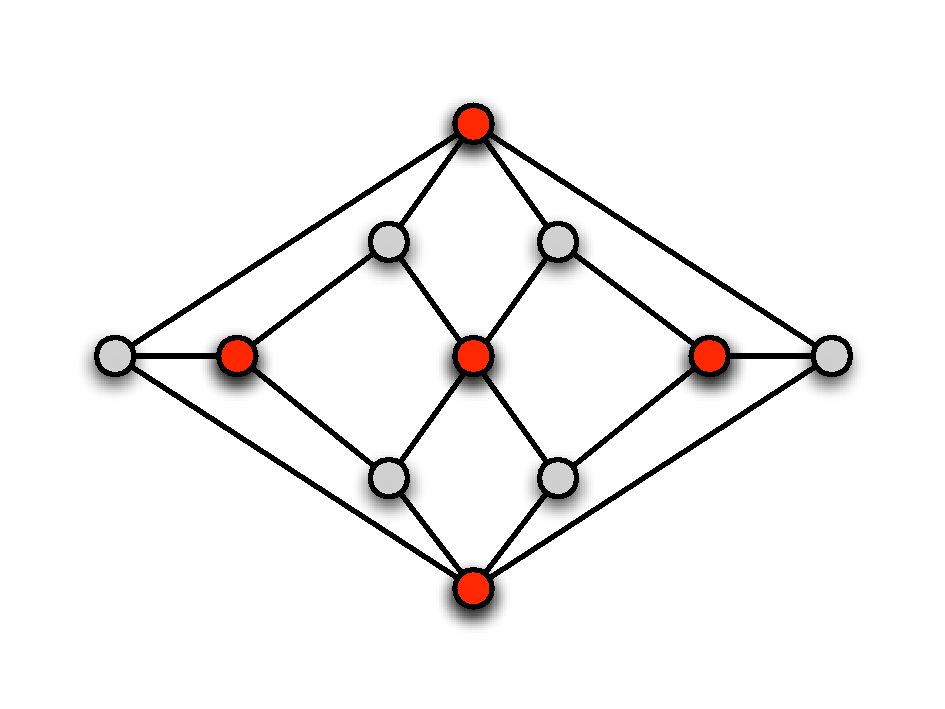
\includegraphics[width=10cm]{pic1.pdf}
    \end{center}
\caption{Herschelov graf, vektorska grafika.}
\label{pic1}
\end{figure}
Pa res lahko vključimo slike katerihkoli formatov? Žal ne. Programski paket \LaTeX\ lahko uporabljamo v več dialektih. Ukaz {\tt latex} ne mara vključenih slik v formatu Portable Document Format {\tt .pdf}, ukaz {\tt pdflatex} pa ne prebavi slik v Encapsulated Postscript Formatu {\tt .eps}.
Strnjeno v Tabeli~\ref{tbl:1}.

\begin{table}
\caption{}
    \begin{center}
        \begin{tabular}{l|ccc}
            ukaz/format & {\tt .pdf} & {\tt .eps} & ostali formati \\ \hline
                        {\tt pdflatex} & da & ne & da \\
                        {\tt latex}   & ne & da  & da
        \end{tabular}
    \end{center}
\label{tbl:1}
\end{table}

Nasvet? Odločite se za uporabo ukaza {\tt pdflatex}. Vaš izdelek bo brez vmesnih stopenj na voljo v {.pdf} formatu in ga lahko odnesete v vsako tiskarno. Če morate na vsak način vključiti sliko, ki jo imate v {\tt .eps} formatu, jo vnaprej pretvorite v alternativni format, denimo {\tt .pdf}.

Včasih se da v okolju za uporabo programskega paketa \LaTeX\ nastaviti na kakšen način bomo prebavljali vhodne dokumente. Spustni meni na Sliki~\ref{pic2} odkriva uporabo \LaTeX{}a v njegovi pdf inkarnaciji --- {\tt pdflatex}.
\begin{figure}
\begin{center}

\includegraphics[width=10cm]{pic2.png}
\end{center}
\caption{Kateri dialekt uporabljati?}
\label{pic2}
\end{figure}
Vključena Slika~\ref{pic2} je seveda bitna.



%----------------------------------------------------------------
% Poglavje (Chapter) 4
%----------------------------------------------------------------
\chapter{Razno}
\label{ch:razno}

\section{Notacije}
\label{sec:notacije}

Za notacijo spremenljivk ter skalarjev uporabimo običajno notacijo, t.j., spremenljivka $x$ in skalar $a$. Pri notaciji matrik ter vektorjev pa se poslužujemo krepega fonta. Torej, matrika $\boldsymbol{A}$ ter vektor $\boldsymbol{v}$,
\begin{equation}
\boldsymbol{A} = \begin{bmatrix}
       a_{11} & a_{12} & \dots & a_{1q}  \\
       a_{21} & a_{22} & \dots & a_{2q}  \\
       \vdots  \\
       a_{p1} & a_{p2} & \dots & a_{pq}  \\
     \end{bmatrix}, \quad
     \boldsymbol{v} = \begin{bmatrix}
       x_1  \\
       x_2  \\
       \vdots  \\
       x_q  \\
     \end{bmatrix}. \nonumber
\end{equation}

%----------------------------------------------------------------
\section{Lepe tabele in psevdokoda}
\label{sec:psevdokoda}

Psevdokoda~\ref{alg:primer} prikazuje primer delovanja genetskega algoritma, medtem ko Tabela~\ref{tab:params} prikazuje primer lepe tabele brez vertikalnih črt.

\begin{algorithm}
\caption{Psevdokoda genetskega algoritma}
\label{alg:primer}
\begin{algorithmic}[1]
\footnotesize
\STATE $t \gets 0$
\STATE $InitPopulation[P(t)] \gets$ inicializiraj populacijo
\STATE $EvalPopulation[P(t)] \gets$ evaluiraj populacijo
\REPEAT
\STATE $P'(t) \gets Variation[P(t)] \gets $ generiraj novo populacijo
\STATE $EvalPopulation[P'(t)] \gets$ evaluiraj novo populacijo
\STATE $P(t+1) \gets ApplyGeneticOperators[P'(t) \in Q]$
\STATE $t \gets t+1$
\UNTIL{prekinitev}
\IF{rezultat dovolj dober}
\STATE shrani rezultat
\ENDIF
\end{algorithmic}
\end{algorithm}

%---------------------------------------------------------------
\begin{table}
\caption{Primer enostavne tabele.}
\centering
\scalebox{0.82}{
\begin{tabular}{c c c}
 \toprule
 Ime & Vrednost & Opis \\
 \midrule
 \textit{ $a$ } & 0.03 &  skalar \\
 \textit{ $x$ } & -1 & spremenljivka \\
 \bottomrule
\end{tabular}
}
\label{tab:params}
\end{table}

%----------------------------------------------------------------
% Poglavje (Chapter) 5
%----------------------------------------------------------------
\chapter{Kaj pa literatura?}
\label{ch3}
% Kot smo omenili že v uvodu, je pravi način za citiranje literature uporaba % \BibTeX{}a~\cite{ubi}.
% Programski paket \LaTeX je prvotno predstavljen v priročniku~\cite{Lamport} % in je v resnici nadgradnja sistema \TeX\ avtorja Donalda Knutha, znanega po % denimo, če izpustim njegovo umetnost programiranja, Knuth-Bendixovem % algoritmu~\cite{Knuth}.
% 
% Vsem raziskovalcem s področja računalništva pa svetujem v branje mnenje L.\ % Fortnowa~\cite{Fortnow}.

%----------------------------------------------------------------
% Poglavje (Chapter) 6
%----------------------------------------------------------------
\chapter{Sklepne ugotovitve}
Izbira \LaTeX\ ali ne \LaTeX\ je seveda prepuščena vam samim. Res je, da so prvi koraki v \LaTeX{}u težavni. Ta dokument naj vam služi kot začetna opora pri hoji.

\fi





%----------------------------------------------------------------
% Poglavje (Chapter) 1
%----------------------------------------------------------------
\chapter{Uvod}
\label{ch:uvod}%solid

\section{Opis problema}
\label{sec:opis-problema}%solid

V železniškem prometu je zagotavljanje varnosti v predorih ključnega pomena, še posebej pri dolgi in široki tovorni kompoziciji, ki se giblje skozi ozke in ukrivljene predore. Problem, ki ga obravnavam v tej magistrski nalogi, je zaznavanje morebitnih trkov med vlakom in stenami predora, ki nastanejo zaradi nepravilnega sledenja predpisanemu varnostnemu prostoru ali napak v modeliranju geometrije predora.

Klasične metode, kot je uporaba minimalnega prereza, so v takšnih scenarijih nezadostne, saj ne upoštevajo kompleksne ukrivljenosti poti ali relativnih premikov vagona, ki lahko presežejo varnostne meje, zlasti v ostrih ovinkih. Problem je izrazit pri dolgi tovorni kompoziciji, kjer razlika med položajem sprednje in zadnje osi povečuje tveganje za trk. Poleg tega trenutne metode pogosto niso dovolj prilagodljive za različne geometrije predorov in vlakov.


\section{Motivacija in cilji dela}
\label{sec:motivacija-cilji}%solid

Motivacija za delo izhaja iz realnega izziva, ki sem ga prejel od podjetja Slovenske železnice. Ti so izrazili potrebo po razvoju avtomatiziranega sistema, ki bi omogočil natančno zaznavanje trkov med vlakom in predorom. 

V tej nalogi predlagam pristop, ki temelji na obdelavi oblaka točk predora in analitičnem modeliranju gibanja vlaka. Osnovna vhodna podatka sta oblak točk predora, pridobljen s 3D laserskim skenerjem, in kontrolne točke, ki definirajo pot železniške proge. Na podlagi teh podatkov sistem obdela geometrijo predora, generira B-zlepke za stene predora v različnih horizontalnih plasteh ter simulira gibanje vagona vzdolž kontrolnih točk. Med simulacijo se izvaja zaznavanje trkov s preverjanjem razdalj med kritičnimi točkami vagona in stenami predora.

Naloga se umešča na področje računalniškega modeliranja in analize v prostoru ter prinaša novost v kombinaciji obdelave oblakov točk s simulacijo gibanja vlaka in zaznavanjem trkov v realnem času.



\section{Prispevki magistrske naloge}
\label{sec:prispevki}%solid

Magistrska naloga bo prispevala k razvoju sistema za zaznavanje trkov med vlakom in predorom s simulacijo gibanja vlaka. V primerjavi z obstoječimi metodami, ki temeljijo na statični analizi minimalnih prerezov, predlagana rešitev omogoča dinamično simulacijo gibanja in kontinuirano preverjanje varnostnih razdalj.

Novost naloge je v integraciji obdelave oblakov točk predora z analitičnim modeliranjem gibanja vagona vzdolž ukrivljene poti ter implementaciji sistema za zaznavanje trkov v realnem času. Glavni prispevki magistrske naloge so:

\begin{itemize}
\item Razvoj sistema za obdelavo oblakov točk predora z B-zlepki za reprezentacijo sten
\item Implementacija simulacije gibanja vagona vzdolž kontrolnih točk z ortogonalnim koordinatnim sistemom
\item Sistem za zaznavanje trkov z analizo razdalj med kritičnimi točkami vagona in stenami predora
\item Praktična aplikacija za Slovenske železnice z možnostjo nadaljnjega razvoja
\end{itemize}



\section{Struktura magistrske naloge}
\label{sec:struktura}%TODO


%----------------------------------------------------------------
% Poglavje (Chapter) 2
%----------------------------------------------------------------
\chapter{Pregled sorodnih del}
\label{ch:pregled-sorodnih-del}%solid

\section{Zaznavanje trkov v prostoru}
\label{sec:zaznavanje-trkov}%solid

Na področju zaznavanja trkov v prostoru se pogosto uporabljajo metode, ki temeljijo na analizi oblakov točk in algoritmih prostorskega indeksiranja. Ena izmed najpogosteje uporabljenih tehnik je uporaba k-d dreves za učinkovito iskanje sosednjih točk v prostoru, kot je prikazano v delu Schauerja in Nüchterja~\cite{Schauer2014}. Prednost njihovega pristopa je visoka računska učinkovitost pri analizi oblakov točk velikega obsega. Ker pa je točk zelo veliko, se poraja potreba po bolj pametnih izračunih trkov. Njihov članek bo služil kot osnova za to magistrsko delo.

Kot alternativo klasičnim metodam so Hermann et al.~\cite{hermann2014} razvili algoritme, ki temeljijo na vokselizaciji prostora. Ti algoritmi omogočajo hitro preverjanje prostorske zasedenosti, vendar lahko pri zelo natančnih analizah izgubijo detajle zaradi diskretizacije prostora.

V delu Niwa in Masuda~\cite{niwa2016} je predstavljen pristop za zaznavanje trkov z metodo globinskih slik, kar izboljša učinkovitost in pravilnost. Ta pristop omogoča zanesljivejše zaznavanje trkov v gostih oblakih točk, vendar ima še vedno veliko časovno in prostorsko zahtevnost.

\section{Obdelava oblakov točk}
\label{sec:obdelava-oblakov}%solid

Klein in Zachmann~\cite{klein-2004-point} obravnavata zaznavanje trkov s pomočjo implicitnih površin, ustvarjenih iz oblakov točk. Njihov pristop je posebej uporaben pri obdelavi kompleksnih geometrij, vendar je računsko zahteven, kar lahko omejuje uporabo v realnem času.

Avtorji Li et al.~\cite{li2020} pregledajo najnovejše pristope strojnega učenja za obdelavo LiDAR podatkov. Izpostavljajo, kako lahko globoko učenje izboljša zaznavanje in analizo oblakov točk v avtonomnih vozilih, še posebej pri neenakomernih in šumnih podatkih. Kljub napredku se metode soočajo z izzivi pri obdelavi velikih oblakov točk in zagotavljanjem rezultatov v realnem času, kar omejuje njihovo uporabnost v hitro spreminjajočih se okoljih.

\section{Metode prostorskega indeksiranja}
\label{sec:prostorsko-indeksiranje}%solid

Prostorsko indeksiranje je ključno za učinkovito obdelavo velikih oblakov točk. K-d drevesa, kot jih uporabljajo Schauer in Nüchter~\cite{Schauer2014}, omogočajo hitro iskanje najbližjih sosedov v večdimenzionalnih prostorih. Te strukture podatkov so posebej primerne za aplikacije, kjer je potrebno pogosto iskanje točk v določeni okolici.

Vendar pa tradicionalne metode prostorskega indeksiranja pogosto niso optimalne za dinamične scenarije, kjer se objekti gibljejo skozi prostor. V takšnih primerih je potreben pristop, ki upošteva časovno komponento gibanja.

\section{Analitično modeliranje v železniškem prometu}
\label{sec:analiticno-modeliranje}

Everett et al.~\cite{Everett_2021} predstavijo sistem za izogibanje trkom v dinamičnih okoljih z uporabo globokega spodbujevalnega učenja. Prednost tega pristopa je prilagodljivost za različne scenarije in obdelava spremenljivega števila agentov brez strogih predpostavk o njihovem gibanju. Kljub temu metoda manj poudarja analizo geometrijskih lastnosti, kar jo omejuje pri natančnih prostorskih analizah, kot je analiza trkov med vlakom in predorom, zaradi česar je njena uporaba v tem kontekstu manj primerna.

\section{Prehodne krivulje v železniškem prometu}
\label{sec:prehodne-krivulje}%solid

V železniškem prometu so prehodne krivulje ključne za zagotavljanje gladkega prehoda med ravnimi in ukrivljenimi odseki prog. Brustad in Dalmo~\cite{infrastructures5050043} analizirajo prehodne krivulje, ki omogočajo gladek prehod med ravnimi in ukrivljenimi odseki železniških tirov. Glavna prednost teh krivulj je njihova sposobnost zmanjšanja sil in obrabe vozil ter tirnic, kar povečuje udobje potnikov in zmanjšuje stroške vzdrževanja. Kljub temu se raziskave na tem področju še vedno soočajo z izzivi, kot so določanje optimalnih lastnosti krivulj za različne scenarije in vozne profile.

Jiang et al.~\cite{s24134403} predlagajo uporabo paraboličnih in sinusoidnih prehodnih krivulj za zmanjšanje dolgovalovnih nepravilnosti v vertikalnih profilih tirov. Prednost tega pristopa je zmanjšanje pospeškov pri prehodih, kar izboljša stabilnost vlaka in varnost potnikov. Slabost pa je, da metoda zahteva precizno načrtovanje in prilagoditev specifičnim konstrukcijskim zahtevam, kar lahko poveča začetne stroške implementacije.

\section{Primerjava obstoječih pristopov}
\label{sec:primerjava-pristopov}%solid

Iz zgoraj predstavljenih del je razvidno, da večina obstoječih metod bodisi zanemarja dinamične lastnosti gibanja bodisi ne omogoča učinkovitega prilagajanja različnim geometrijam. Metode, ki temeljijo na obdelavi oblakov točk~\cite{Schauer2014, niwa2016}, so računsko zahtevne in pogosto niso primerne za analizo v realnem času. Po drugi strani pristopi strojnega učenja~\cite{li2020, Everett_2021} omogočajo prilagodljivost, vendar ne zagotavljajo teoretično podprtih rezultatov, ki so potrebni za varnostno kritične aplikacije v železniškem prometu.

Cilj te magistrske naloge je preseči omejitve obstoječih pristopov z vključitvijo analitičnega modeliranja gibanja kritičnih točk in prekrivanjem teh krivulj z geometrijo predora, kar bo omogočilo natančnejše in hitrejše zaznavanje trkov.




%----------------------------------------------------------------
% Poglavje (Chapter) 3
%----------------------------------------------------------------
\chapter{Teoretične osnove}
\label{ch:teoreticne-osnove}

V tem poglavju predstavimo teoretične osnove, ki so potrebne za razumevanje predlaganega pristopa k zaznavanju trkov med vlakom in predorom. Osredotočimo se na geometrijsko predstavitev objektov v prostoru, matematične osnove B-zlepkov ter algoritme za zaznavanje trkov.

\section{Geometrijska predstavitev predorov}
\label{sec:geometrijska-predstavitev-predorov}%solid

Predori so predstavljeni z oblaki točk, pridobljenih s 3D laserskim skenerjem. Oblak točk predstavlja diskretno vzorčenje površine predora, kjer vsaka točka $\boldsymbol{p}_i = (x_i, y_i, z_i)$ določa prostorsko pozicijo na steni predora. Oblak točk $\mathcal{P} = \{\boldsymbol{p}_1, \boldsymbol{p}_2, \ldots, \boldsymbol{p}_n\}$ vsebuje $n$ točk, ki skupaj opisujejo geometrijo predora.

V našem pristopu obravnavamo podatke predorov, ki so organizirani kot zaporedni prečni prerezi vzdolž osi predora. Vsak presek je definiran z množico 2D koordinat $(x, y)$, ki opisujejo obris predora na določeni poziciji vzdolž osi $z$.

Glavni izziv pri obdelavi takšnih podatkov je njihova transformacija v uporaben 3D oblak točk, ki ohranja geometrijske lastnosti predora. To dosežemo z naslednjim pristopom:

\begin{itemize}
    \item \textbf{Postavitev oblaka točk v 3D}: 2D koordinate $(x, y)$ za vsak presek dopolnimo z $z$ koordinato, ki ustreza poziciji vzdolž poti
    \item \textbf{Transformacija koordinatnega sistema}: podatki se transformirajo iz globalnega koordinatnega sistema v lokalni koordinatni sistem predora, kjer $z$-os sovpada s središčno linijo predora
\end{itemize}

Matematična formulacija transformacije je podana z:

\begin{equation}
\boldsymbol{p}'_i = \boldsymbol{R}(\boldsymbol{p}_i - \boldsymbol{t}_{\text{center}})
\label{eq:coordinate-transform}
\end{equation}

kjer je $\boldsymbol{R}$ rotacijska matrika, izpeljana iz tangentnega vektorja središčne linije, $\boldsymbol{t}_{\text{center}}$ pa translacijski vektor do središča predora. 

Za konstrukcijo rotacijske matrike $\boldsymbol{R}$ uporabimo Rodriguesovo rotacijsko formulo~\cite{DAI2015144}:

\begin{equation}
\boldsymbol{R} = \boldsymbol{I} + \sin(\theta) \boldsymbol{K} + (1 - \cos(\theta)) \boldsymbol{K}^2
\end{equation}

kjer je $\theta$ kot med vektorjema, $\boldsymbol{K}$ pa antisimetrična matrika osi rotacije. Namen te transformacije je prilagoditi oblak točk dejanskemu poteku predora v prostoru. Ker so prvotni podatki organizirani kot ravni prerezi, rotacijska transformacija zagotovi, da se oblak točk čim bolje prilega dejanski ukrivljeni geometriji predora. To je ključno za natančno predstavitev prostorskih odnosov med vlakom in stenami predora ter posledično za zanesljivo zaznavanje trkov.

\section{Geometrijski model vagona}
\label{sec:geometrijski-model-vagona}

Vagon je modeliran kot pravokotno telo (kvader) z dimenzijami širina $w$, višina $h$ in globina $d$. Geometrijska predstavitev temelji na konceptu medosne razdalje in ortogonalnem koordinatnem sistemu.

\subsection{Pozicioniranje z medosno razdaljo}%solid
\label{subsec:pozicioniranje-medosje}

Pozicija vagona je določena s točkama $\boldsymbol{p}_0$ in $\boldsymbol{p}_1$, ki sta oddaljeni za medosno razdaljo $l_{wb}$. Za določitev sprednje osi uporabljamo metodo presečišča kroga in krivulje.

Sprednja os $\boldsymbol{p}_1$ se nahaja na presečišču kroga s središčem v $\boldsymbol{p}_0$ in radijem $l_{wb}$ z B-zlepkem kontrolnih točk:

\begin{equation}
\|\boldsymbol{C}(t) - \boldsymbol{p}_0\|^2 = l_{wb}^2
\label{eq:circle-curve-intersection}
\end{equation}

kjer je $\boldsymbol{C}(t)$ parametrična predstavitev B-zlepka kontrolnih točk in $t \in [0,1]$ parameter krivulje.

Za rešitev te enačbe iščemo ničle funkcije:

\begin{equation}
f(t) = \|\boldsymbol{C}(t) - \boldsymbol{p}_0\|^2 - l_{wb}^2
\label{eq:intersection-function}
\end{equation}

Ta pristop zagotavlja, da je medosna razdalja natančno ohranjena tudi na ukrivljenih odsekih poti, kar je ključno za realistično modeliranje gibanja vagona.

\subsection{Ortogonalni koordinatni sistem}%solid
\label{subsec:ortogonalni-sistem-vagon}

Orientacija vagona v prostoru je določena z ortogonalnim koordinatnim sistemom:

\begin{align}
\boldsymbol{f} &= \frac{\boldsymbol{p}_1 - \boldsymbol{p}_0}{\|\boldsymbol{p}_1 - \boldsymbol{p}_0\|} \quad \text{(naprej)} \\
\boldsymbol{u} &= (0, 1, 0) \quad \text{(navzgor)} \\
\boldsymbol{r} &= \boldsymbol{u} \times \boldsymbol{f} \quad \text{(desno)}
\label{eq:wagon-frame}
\end{align}

\subsection{Simulacija premika vagona}%solid
\label{subsec:simulacija-premika-vagona}

Za potrebe simulacije gibanja vagona je potrebno določiti celoten geometrijski model, ki omogoča natančno predstavitev vagona v prostoru. Vagon je modeliran z osmimi vogali pravokotnega telesa, ki se izračunajo na podlagi dejanskih mej vagona.

Najprej definirajmo sprednjo in zadnjo mejo vagona:

\begin{align}
\boldsymbol{p}_{\text{rear}} &= \boldsymbol{p}_0 - \boldsymbol{f} \cdot (d \cdot \omega) \\
\boldsymbol{p}_{\text{front}} &= \boldsymbol{p}_0 + \boldsymbol{f} \cdot (d \cdot (1 - \omega))
\label{eq:wagon-actual-ends}
\end{align}

kjer je $\omega$ parameter odmika koles, $d$ globina vagona in $\boldsymbol{f}$ enotski vektor v smeri naprej.

Osem vogalov vagona je nato definiranih kot:

\begin{equation}
\boldsymbol{v}_{i,j,k} = \boldsymbol{p}_{\text{base}} + i \cdot \frac{w}{2} \boldsymbol{r} + j \cdot h \cdot \boldsymbol{u} + k \cdot \frac{d}{2} \cdot \boldsymbol{f}
\label{eq:wagon-vertices}
\end{equation}

kjer so $i, k \in \{-1, 1\}$, $j \in \{0, 1\}$ in $\boldsymbol{p}_{\text{base}} = \frac{\boldsymbol{p}_{\text{rear}} + \boldsymbol{p}_{\text{front}}}{2}$ je središče med zadnjo in sprednjo mejo vagona.

Ta pristop omogoča popolno geometrijsko predstavitev vagona v prostoru ter je ključen za vizualizacijo in analizo gibanja celotne strukture vagona vzdolž ukrivljene poti.

\subsection{Kritične točke za računanje trkov}%solid
\label{subsec:kriticne-tocke-racunanje-trkov}

Za učinkovito zaznavanje trkov se na vsaki višinski ravnini $y$ v predoru uporablja optimiziran nabor šestih kritičnih točk, ki predstavljajo najkritičnejše pozicije za možne kolizije s stenami. Te točke so razporejene v treh vzdolžnih pozicijah (zadaj, sredina, spredaj) na obeh stranskih robovih vagona.

Kritične točke za zaznavanje kolizij na višini $y$ so definirane s formulo:

\begin{equation}
\boldsymbol{c}_{s,p} = \boldsymbol{p}_{base,p} + s \cdot \frac{w}{2} \boldsymbol{r} + y \cdot \boldsymbol{u}
\label{eq:critical-points-wagon}
\end{equation}

kjer je:
\begin{align}
s &\in \{-1, 1\} \quad \text{(levo/desno)} \nonumber \\
p &\in \{\text{back}, \text{middle}, \text{front}\} \quad \text{(zadaj, sredina, spredaj)} \nonumber \\
\boldsymbol{p}_{base,back} &= \boldsymbol{p}_{\text{rear}} \nonumber \\
\boldsymbol{p}_{base,middle} &= \frac{\boldsymbol{p}_{\text{rear}} + \boldsymbol{p}_{\text{front}}}{2} \nonumber \\
\boldsymbol{p}_{base,front} &= \boldsymbol{p}_{\text{front}} \nonumber
\end{align}

kjer je $\boldsymbol{r}$ enotski vektor v desno smer, $\boldsymbol{u}$ enotski vektor navzgor in $w$ širina vagona.

Ta pristop generira za vsako horizontalno ravnino predora (definirano z $y$ koordinato) natanko šest kritičnih točk, ki pokrivajo celotno širino in dolžino vagona. Sistematična razporeditev omogoča zanesljivo zaznavanje kršitev varnostnih razdalj ali situacij, kjer bi se vagon nahajal zunaj dovoljenih mej predora.




\section{B-zlepki (B-splines)}
\label{sec:b-zlepki}

B-zlepki so parametrične krivulje, ki omogočajo gladko interpolacijo ali aproksimacijo množice točk. V našem sistemu jih uporabljamo za reprezentacijo sten predora ter za modeliranje poti vagona.

\subsection{Matematične osnove B-zlepkov}
\label{subsec:matematicne-osnove-b-zlepkov}

B-zlepek stopnje $p$~\cite{b_splines} je definiran s kontrolnimi točkami $\boldsymbol{C}_0, \boldsymbol{C}_1, \ldots, \boldsymbol{C}_n$ in vozliščnim vektorjem $\boldsymbol{t} = \{t_0, t_1, \ldots, t_{n+p+1}\}$:

\begin{equation}
\boldsymbol{S}(y) = \sum_{i=0}^{n} \boldsymbol{C}_i B_{i,p}(y)
\label{eq:b-spline}
\end{equation}

kjer so $B_{i,p}(y)$ B-zlepek bazne funkcije, definirane rekurzivno:

\begin{align}
B_{i,0}(y) &= \begin{cases}
1 & \text{če } t_i \leq y < t_{i+1} \\
0 & \text{sicer}
\end{cases} \\
B_{i,p}(y) &= \frac{y - t_i}{t_{i+p} - t_i} B_{i,p-1}(y) + \frac{t_{i+p+1} - y}{t_{i+p+1} - t_{i+1}} B_{i+1,p-1}(y).
\label{eq:b-spline-basis}
\end{align}


\subsection{Interpolacija in aproksimacija}
\label{subsec:interpolacija-aproksimacija}

Pri obdelavi oblakov točk predora uporabljamo dva pristopa:

\textbf{Interpolacija}: B-zlepek natančno prehaja skozi vse podane točke. To je ustrezno, ko želimo ohraniti vse detajle geometrije predora.

\textbf{Aproksimacija}: B-zlepek se prilagodi splošni obliki podatkov, vendar ne prehaja natančno skozi vse točke. To je koristno za zmanjšanje vpliva šuma v meritvah.



\section{Metode za merjenje razdalj in določanje strani}
\label{sec:metode-razdalj}

Za zaznavanje trkov je ključno merjenje razdalj med točkami vagona in stenami predora ter določanje, na kateri strani B-zlepka se točka nahaja.

\subsection{Razdalja do parametrične krivulje}
\label{subsec:razdalja-krivulja}

Razdalja med točko $\boldsymbol{q}$ in B-zlepkom $\boldsymbol{C}(u)$ je definirana kot:

\begin{equation}
d(\boldsymbol{q}, \boldsymbol{C}) = \min_{u \in [0,1]} \|\boldsymbol{q} - \boldsymbol{C}(u)\|
\label{eq:distance-spline}
\end{equation}

To je optimizacijski problem, ki ga rešujemo numerično z iskanjem najbližje točke na krivulji.

\subsection{Določanje strani}
\label{subsec:dolocanje-strani}

Za določitev, ali se točka nahaja znotraj ali zunaj predora, uporabljamo predznak razdalje. Za 2D preseku predora uporabimo vektorski produkt za določitev strani:

\begin{equation}
s = \text{sign}(\boldsymbol{t} \times (\boldsymbol{q} - \boldsymbol{C}(u^*)))
\label{eq:side-determination}
\end{equation}

kjer pozitivni predznak pomeni, da je točka na levi strani krivulje, negativni pa na desni.



%----------------------------------------------------------------
% Poglavje (Chapter) 4
%----------------------------------------------------------------
\chapter{Metodologija in pristop}
\label{ch:metodologija}

\section{Pregled predlaganega pristopa}
\label{sec:pregled-pristopa}

Pri magistrski nalogi se osredotočam na pristop k zaznavanju trkov med vlakom in predorom, ki vključuje več korakov. Kot vhodni podatki se uporabljajo oblaki točk predora, pridobljeni s 3D laserskim skenerjem, ter kontrolne točke, ki definirajo pot železniške proge.

Metodologija vključuje obdelavo oblakov točk predora s transformacijo vzdolž ukrivljene poti, generiranje horizontalnih prerezov predora z B-zlepki za reprezentacijo sten, modeliranje vagona kot kvadra ter simulacijo gibanja vagona vzdolž kontrolnih točk. Med simulacijo se izvaja zaznavanje trkov s preverjanjem razdalj med kritičnimi točkami vagona in stenami predora z določenim varnostnim odmikom.

Sistem je implementiran v programskem jeziku Python z uporabo knjižnic PyVista za vizualizacijo, NumPy za numerične izračune in SciPy za interpolacijo z B-zlepkami.


\section{Predobdelava vhodnih podatkov}
\label{sec:predobdelava}

\subsection{Obdelava oblakov točk predora}
\label{subsec:obdelava-oblakov-predor}

\subsection{Modeliranje vagona}
\label{subsec:modeliranje-vagona}

\subsection{Obdelava kontrolnih točk}
\label{subsec:obdelava-kontrolnih-tock}

\section{Generiranje kontrolnih točk}
\label{sec:generiranje-kontrolnih}

\section{Modeliranje gibanja vagona}
\label{sec:modeliranje-gibanja-vagona}

\subsection{Izračun pozicije na osnovi medosne razdalje}
\label{subsec:izracun-pozicije-medosje}

\subsection{Določitev kritičnih točk vagona}
\label{subsec:kriticne-tocke}

\subsection{Izračun krivulj gibanja}
\label{subsec:krivulje-gibanja}

\section{Algoritmi za zaznavanje trkov}
\label{sec:algoritmi-zaznavanje}

Zaznavanje trkov temelji na preverjanju dveh pogojev: ali se kritične točke vagona nahajajo preblizu stenami predora (kršitev varnostnega odmika) ali zunaj predora.

\subsection{Varnostni odmik}
\label{subsec:varnostni-odmik}

Varnostni odmik $\delta$ predstavlja minimalno dovoljeno razdaljo med vagom in steno predora. Kršitev nastane, ko:

\begin{equation}
d(\boldsymbol{v}_i, \boldsymbol{C}_{\text{stena}}) < \delta
\label{eq:safety-violation}
\end{equation}

kjer je $\boldsymbol{v}_i$ kritična točka vagona in $\boldsymbol{C}_{\text{stena}}$ B-zlepek stene predora.

\subsection{Algoritem zaznavanja}
\label{subsec:algoritem-zaznavanja}

Glavni algoritem zaznavanja trkov deluje v naslednjih korakih:
\begin{enumerate}
    \item Za vsako kritično točko vagona $\boldsymbol{v}_i$
    \item Izračunaj razdaljo do leve stene $d_L$ in desne stene $d_R$
    \item Določi, na kateri strani sten se točka nahaja
    \item Preverti kršitve:
        \begin{itemize}
            \item Če $d_L < \delta$ ali $d_R < \delta$: kršitev varnostnega odmika
            \item Če je točka na napačni strani: zunaj predora
        \end{itemize}
\end{enumerate}


Psevdokoda algoritma je predstavljena v Algoritmu~\ref{alg:collision-detection}.

\begin{algorithm}
\caption{Zaznavanje trkov med vagom in predorom}
\label{alg:collision-detection}
\begin{algorithmic}[1]
\footnotesize
\STATE $\text{violations} \gets \emptyset$
\FOR{vsako kritično točko $\boldsymbol{v}_i$ vagona}
    \STATE $d_L \gets$ razdalja od $\boldsymbol{v}_i$ do leve stene
    \STATE $d_R \gets$ razdalja od $\boldsymbol{v}_i$ do desne stene
    \STATE $s_L \gets$ stran glede na levo steno
    \STATE $s_R \gets$ stran glede na desno steno
    \IF{$d_L < \delta$}
        \STATE dodaj kršitev: "preblizu levi steni"
    \ENDIF
    \IF{$d_R < \delta$}
        \STATE dodaj kršitev: "preblizu desni steni"
    \ENDIF
    \IF{$s_L < 0$ ali $s_R > 0$}
        \STATE dodaj kršitev: "zunaj predora"
    \ENDIF
\ENDFOR
\RETURN $\text{violations}$
\end{algorithmic}
\end{algorithm}

%----------------------------------------------------------------
% Poglavje (Chapter) 5
%----------------------------------------------------------------
\chapter{Implementacija}
\label{ch:implementacija}

\section{Arhitektura sistema}
\label{sec:arhitektura}

\section{Ključni moduli implementacije}
\label{sec:kljucni-moduli}

\subsection{TunnelSlicer -- obdelava geometrije predora}
\label{subsec:tunnel-slicer}

\subsection{TrainGenerator -- modeliranje vlaka}
\label{subsec:train-generator}

\subsection{CollisionDetector -- zaznavanje trkov}
\label{subsec:collision-detector}

\subsection{Simulation -- simulacija gibanja}
\label{subsec:simulation}

\section{B-zlepki za stene predora}
\label{sec:b-zlepki-stene}

\section{Transformacije koordinatnih sistemov}
\label{sec:transformacije-koordinatni}

\section{Simulacija gibanja vagona}
\label{sec:simulacija-gibanja}

\section{Vizualizacija simulatorja}
\label{sec:vizualizacija}

%----------------------------------------------------------------
% Poglavje (Chapter) 6
%----------------------------------------------------------------
\chapter{Eksperimentalno ovrednotenje}
\label{ch:eksperimentalno-ovrednotenje}

\section{Testni scenariji in podatki}
\label{sec:testni-scenariji}

\subsection{Predor Ringo}
\label{subsec:predor-ringo}

\subsection{Predor Globoko}
\label{subsec:predor-globoko}

\section{Parametri sistema}
\label{sec:parametri-sistema}

\section{Evalvacijski kriteriji}
\label{sec:evalvacijski-kriteriji}

Evalvacija sistema je bila izvedena z analizo delovanja na dveh testnih scenarijih. Preverjalo se je pravilno zaznavanje kršitev varnostnih razdalj, stabilnost sistema med simulacijo ter ustreznost vizualizacije rezultatov. Sistem je uspešno zaznal situacije, kjer se vagon približa preblizu stenam predora ali presega dovoljene meje predora.


\section{Rezultati testiranja}
\label{sec:rezultati-testiranja}

\subsection{Natančnost zaznavanja trkov}
\label{subsec:natancnost-zaznavanja}

\subsection{Računska učinkovitost}
\label{subsec:racunska-ucinkovitost}

\subsection{Analiza varnostnih razdalj}
\label{subsec:analiza-varnostnih}

\section{Primerjava z obstoječimi metodami}
\label{sec:primerjava-metode}

\section{Diskusija rezultatov}
\label{sec:diskusija-rezultatov}

%----------------------------------------------------------------
% Poglavje (Chapter) 7
%----------------------------------------------------------------
\chapter{Sklepne ugotovitve}
\label{ch:sklepne-ugotovitve}

\section{Povzetek prispevkov}
\label{sec:povzetek-prispevkov}

\section{Omejitve pristopa}
\label{sec:omejitve}

\section{Predlogi za nadaljnje delo}
\label{sec:predlogi-nadaljnje}

















% ---------------------------------------------------------------
% Appendix
% ---------------------------------------------------------------
%\appendix
%\addcontentsline{toc}{chapter}{Razširjeni povzetek}
%\chapter{Title of the appendix 1}

%Example of the appendix.

%----------------------------------------------------------------
% SLO: bibliografija
% ENG: bibliography
%----------------------------------------------------------------
\bibliographystyle{elsarticle-num}

%----------------------------------------------------------------
% SLO: odkomentiraj za uporabo zunanje datoteke .bib (ne pozabi je potem prevesti!)
% ENG: uncomment to use .bib file (don't forget to compile it!)
%----------------------------------------------------------------
\bibliography{bibliography}

\end{document}
